%\documentclass[12pt]{article}
%\usepackage[a4paper, margin=1in]{geometry} 
%\usepackage{graphicx} 
%\usepackage{hyperref}
%\usepackage{float}
%\usepackage{multicol}
%\usepackage[font=small, labelfont=bf]{caption}
%
%\begin{document}

%
% Local alignments
%
\subsection{Local alignments}
Local pairwise alignments are aligned pairs of sub--sequences that have centain level of similarities.

%
% Deiffrence between global and local alignments
%
\subsubsection*{Deiffrence between global and local alignments} 

\begin{figure}[H]
  \centering
      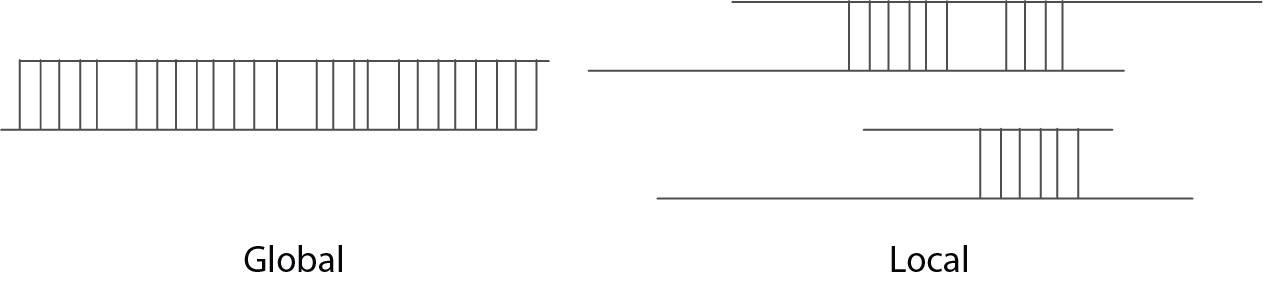
\includegraphics[width=0.75\textwidth]{fig04/global_and_local_alignments.png}
  \caption{Global and local alignments}
\end{figure}

%
% Elements of local alignment
%
\subsubsection*{Elements of local alignment}
\begin{itemize}
\item Segment: a substring of a sequence
\item Segment pair: a pair of segments
\item Local alignment: an alignment of a segment pair
\end{itemize}

%
% Alignment methods
%
\subsubsection*{Elements of local alignment}
\begin{itemize}
\item Dynamic programming (Smith--Waterman)
\item Dot matrix
\end{itemize}

%
% Applications
%
\subsubsection*{Applications}
\begin{itemize}
\item Sequence motifs
\item Conserved regions
\item Inverted repeats
\end{itemize}

\bigskip 

%\end{document}
